\section{Light}

\begin{multicols}{2}


\section*{Propagation of Light}


\subsection{Light Travels in a Straight Line}

\begin{center}
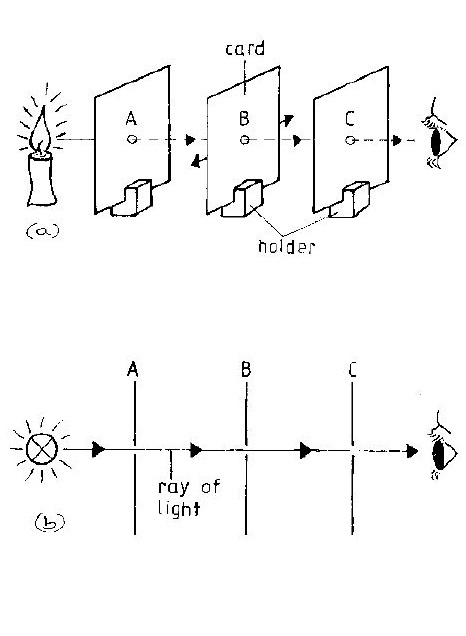
\includegraphics[width=0.49\textwidth]{./img/source/prop-of-light-2.jpg}
\end{center}

\begin{description*}
%\item[Subtopic:]{}
\item[Materials:]{Candle, cardboard/3 toilet paper tubes, nail, string}
\item[Setup:]{Cut 3 rectangular pieces of cardboard or use 3 toilet paper tubes. Poke a hole at the center of each using a nail. The holes should all be equal distance from the bottom.}
\item[Procedure:]{Arrange the cardboard pieces in a straight line - pass a string through the holes and pull tight to do this. Place the candle or light source near card A and look through card C. Displace any of the 3 cards and look again.}
%\item[Hazards:]{}
%\item[Questions:]{}
\item[Observations:]{The light can be seen when all holes are in a straight line, but not when any card is moved.}
\item[Theory:]{Light travels in a straight line. The ray of light cannot be seen through card C when there is an obstruction in its path. Figure (b) shows the \emph{ray diagram} for the path of the light.}
%\item[Applications:]{}
%\item[Notes:]{}
\end{description*}

\vfill
\columnbreak

\subsection{Light Through a Comb}

\begin{center}
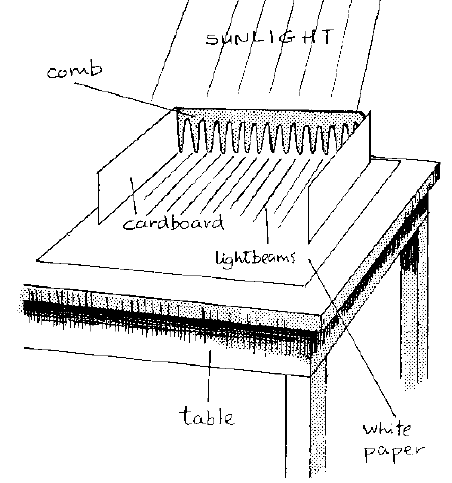
\includegraphics[width=0.45\textwidth]{./img/source/light-comb.png}
\end{center}

\begin{description*}
%\item[Subtopic:]{}
\item[Materials:]{Comb, light source, paper, cardboard}
%\item[Setup:]{}
\item[Procedure:]{Hold a comb on a white paper placed on a table near a window. Place cardboard on either side of the comb.}
%\item[Hazards:]{}
%\item[Questions:]{}
\item[Observations:]{Parallel beams of light can be seen on the paper.}
\item[Theory:]{Light travels in a straight line, so beams of sunlight passing through the slits in the comb appear in parallel lines on the paper.}
%\item[Applications:]{}
%\item[Notes:]{}
\end{description*}

\subsection{Ray Boxes}

\begin{center}
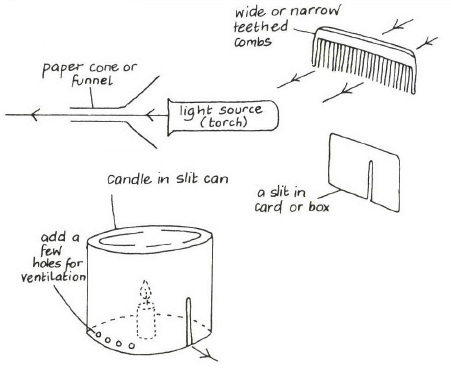
\includegraphics[width=0.49\textwidth]{./img/vso/ray-boxes.jpg}
\end{center}

\begin{description*}
%\item[Subtopic:]{}
\item[Materials:]{Torch, paper funnel, comb, card, tin can, candle}
%\item[Setup:]{}
\item[Procedure:]{Many experiments with light require thin beams of light. Make a ray box using one of the methods shown.}
%\item[Hazards:]{}
%\item[Questions:]{}
%\item[Observations:]{}
%\item[Theory:]{}
%\item[Applications:]{}
%\item[Notes:]{}
\end{description*}

\subsection{Pinhole Camera}

\begin{center}
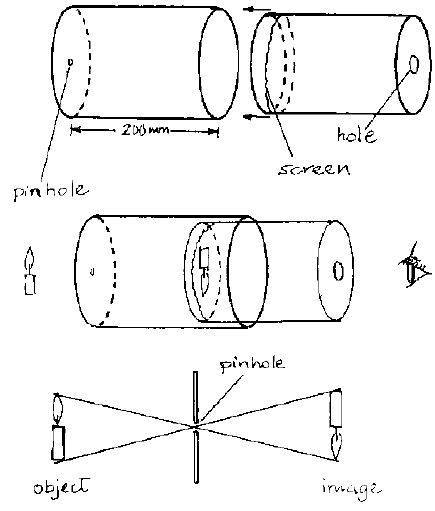
\includegraphics[width=0.4\textwidth]{./img/source/pinhole-camera.png}
\end{center}

\begin{description*}
%\item[Subtopic:]{}
\item[Materials:]{Tin/cardboard box/manila paper, glue, pin, candle}
\item[Setup:]{Roll a piece of manila paper to make a cylinder. Glue a circular piece of card on one end and poke a hole with a pin. Make a second cylinder to fit tightly in the first. Cover one end with plain paper to act as a screen, and close the other end with a card. At the center of the card make a large 2 cm diameter hole.}
\item[Procedure:]{Observe a burning candle by looking through the large hole. Adjust the inner cylinder to get a sharp image. Adjust the distance between screen and pinhole, as well as between candle and pinhole.}
%\item[Hazards:]{}
%\item[Questions:]{}
\item[Observations:]{The image of the candle is real and inverted. When the distance from screen to pinhole is increased, the image becomes larger and more blurred. When the candle is closer to the pinhole, the image gets smaller and sharper.}
\item[Theory:]{The rays of light from the candle cross at the pinhole and thus show up on the screen as an inverted image.}
%\item[Applications:]{}
%\item[Notes:]{}
\end{description*}

\subsection{Transparent, Translucent, Opaque}

%\begin{center}
%\includegraphics[width=0.4\textwidth]{./img/.jpg}
%\end{center}

\begin{description*}
%\item[Subtopic:]{}
\item[Materials:]{Piece of glass/clear plastic, book, paper, oil}
%\item[Setup:]{}
\item[Procedure:]{Hold a clear sheet of glass or plastic up in the light. Hold up a book. Rub some cooking oil on a sheet of paper and hold it up.}
%\item[Hazards:]{}
%\item[Questions:]{}
%\item[Observations:]{}
\item[Theory:]{The glass/plastic is \emph{transparent} - it allows light to pass through it. The book is \emph{opaque} - light does not pass through it. The oily paper is \emph{translucent} - it allows some light to pass through it.}
%\item[Applications:]{}
%\item[Notes:]{}
\end{description*}

\subsection{Formation of Shadows}

\begin{center}
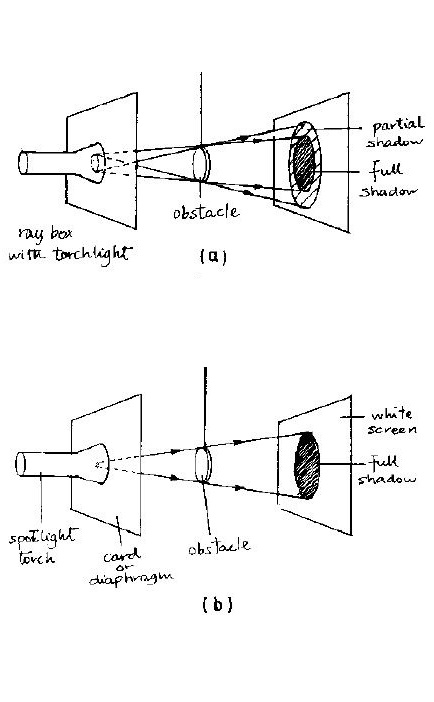
\includegraphics[width=0.49\textwidth]{./img/source/shadows.jpg}
\end{center}

\begin{description*}
%\item[Subtopic:]{}
\item[Materials:]{Torch, cardboard, obstacle (e.g. bucket lid)}
%\item[Setup:]{}
\item[Procedure:]{Place a torch light behind a piece of cardboard with a large hole in it. Hold an obstacle in front of the light (a). Change the hole to a very small size and note the shadow formed by the same obstacle on the same screen (b). Repeat in sunlight.}
%\item[Hazards:]{}
%\item[Questions:]{}
\item[Observations:]{The large hole produces a partial shadow and full shadow, while the small hole produces a full shadow only.}
\item[Theory:]{Extended light sources give partial shadows (called \emph{penumbra}) and full shadows (called \emph{umbra}), while single point sources give mainly full shadows. Sharper shadows are obtained when an
obstacle intercepts parallel rays, i.e. rays from a distant source. }
\item[Applications:]{Though the sun is an
extended source, its rays reach the earth parallel and therefore produce sharp shadows.}
%\item[Notes:]{}
\end{description*}

\vfill
\columnbreak

%==================================================================================================%

\section*{Reflection of Light}


\subsection{Laws of Reflection}
\textbf{*NECTA PRACTICAL*}

\begin{center}
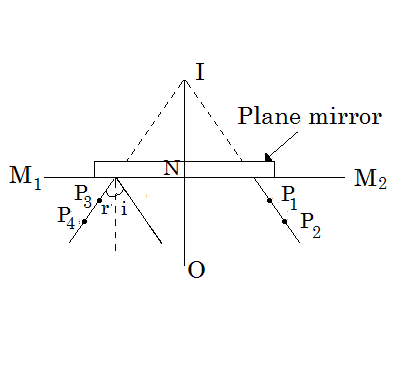
\includegraphics[width=0.49\textwidth]{./img/plane-mirror-prac.png}
\end{center}

\begin{description*}
%\item[Subtopic:]{}
\item[Materials:]{Plane mirror, pins/syringe needles, paper, ruler, protractor}
\item[Setup:]{Attach a plane mirror to a block of wood.}
\item[Procedure:]{Stand up the mirror and trace a straight line along its base. Place a pin at O a few cm from the mirror. Look at the mirror from the right side and place to pins P$_1$ and P$_2$ so that they appear in a straight line with the image. Repeat for the left side using pins P$_3$ and P$_4$. Remove the mirror and pins and join the straight lines to meet at I behind the mirror.}
%\item[Hazards:]{}
\item[Questions:]{Measure and compare the distances ON and NI using a ruler. Measure angles $i$ and $r$ with a protractor.}
\item[Observations:]{The distances ON and NI are equal. The angles $i$ and $r$ are equal.}
\item[Theory:]{The laws of reflection for a plane mirror state that: (1) object distance (ON) and image distance (NI) are equal; and (2) the angle of incidence ($i$) and angle of reflection ($r$) are equal.}
%\item[Applications:]{}
%\item[Notes:]{}
\end{description*}

\vfill
\columnbreak

\subsection{Reversed Image}

\begin{center}
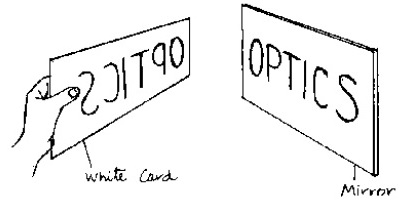
\includegraphics[width=0.4\textwidth]{./img/source/reversed-image-2.jpg}
\end{center}

\begin{description*}
%\item[Subtopic:]{}
\item[Materials:]{Paper, mirror, pen}
%\item[Setup:]{}
\item[Procedure:]{Write the word OPTICS on an ordinary piece of paper. Turn the paper and retrace the faint word appearing on its back. Place the paper in front of a plane mirror.}
%\item[Procedure:]Write the word OPTICS on an ordinary piece of paper (a). Turn the paper and retrace the faint word appearing on its back (b). You will obtain the
%mirror-writing of the word OPTICS. The latter is a reversed image of the former.
%Place the piece of paper in front of a plane mirror (see figure (c)).}
%\item[Hazards:]{}
%\item[Questions:]{}
%\item[Observations:]{}
\item[Theory:]{Mirror images are reversed images, i.e. the left and right side of the object are
interchanged.}
%\item[Applications:]{}
%\item[Notes:]{}
\end{description*}

\subsection{Images Formed in Multiple Mirrors}
\textbf{*NECTA PRACTICAL*}

\begin{center}
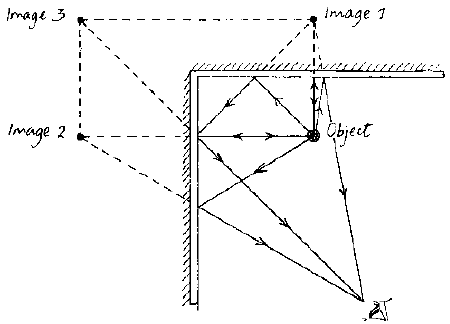
\includegraphics[width=0.45\textwidth]{./img/source/multiple-mirrors.png}
\end{center}

\begin{description*}
%\item[Subtopic:]{}
\item[Materials:]{2 plane mirrors, pin, paper, protractor}
%\item[Setup:]{}
\item[Procedure:]{Place to mirrors upright at right angles to each other. Place a pin (Object) in between them. Look at the mirrors and count the number of images seen. Repeat with mirrors at angles of 60$^\circ$ and 45$^\circ$.}
%\item[Hazards:]{}
\item[Questions:]{How many images can be seen in each case?}
\item[Observations:]{At right angles, 3 images are produced; at 60$^\circ$, 5 images; and at 45$^\circ$, 7 images.}
\item[Theory:]{For an angle $\theta$ between the mirrors, the number of images produced $n$ follows the relationship $n = \frac{360^\circ}{\theta} - 1$.}
\item[Applications:]{Kaleidoscope}
%\item[Notes:]{}
\end{description*}

%==================================================================================================%

\section*{Applications of Reflection}


\subsection{Periscope} \label{sub:i-periscope}

\begin{center}
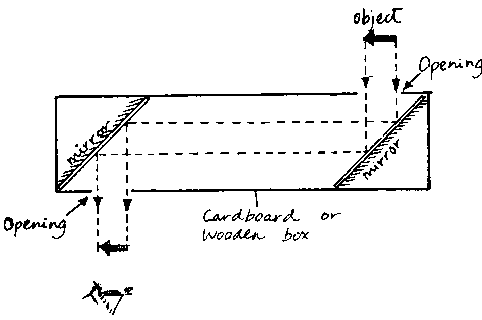
\includegraphics[width=0.49\textwidth]{./img/source/periscope.png}
\end{center}

\begin{description*}
%\item[Subtopic:]{}
\item[Materials:]{2 mirrors, rectangular box, glue/tape, scissors}
\item[Setup:]{Arrange two mirrors in the box as shown. The mirrors should be at 45$^\circ$ angles to the walls. }
\item[Procedure:]{Look through the periscope to view objects above walls and around corners.}
%\item[Hazards:]{}
%\item[Questions:]{}
\item[Observations:]{Images produced are upright.}
%\item[Theory:]{}
\item[Applications:]{Submarines}
%\item[Notes:]{}
\end{description*}

\vfill
\columnbreak

\subsection{Kaleidoscope}

\begin{center}
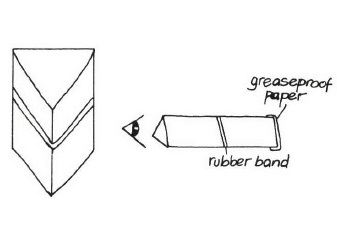
\includegraphics[width=0.45\textwidth]{./img/vso/kaleidoscope.jpg}
\end{center}

\begin{description*}
%\item[Subtopic:]{}
\item[Materials:]{3 mirrors of equal size, tape, cardboard, rubber bands, coloured objects (optional)}
\item[Setup:]{Tape the 3 mirrors together so that they form a triangular tube with the reflective sides facing inwards. Wrap them in cardboard and fix with rubber bands.}
\item[Procedure:]{Look through the kaleidoscope at any objects, especially coloured beads or paper, and turn to watch the colors change.}
%\item[Hazards:]{}
%\item[Questions:]{}
%\item[Observations:]{}
%\item[Theory:]{}
%\item[Applications:]{}
%\item[Notes:]{}
\end{description*}


\end{multicols}

\pagebreak